\documentclass[epsfig]{article}
\usepackage{epsfig}
\usepackage{amsmath}
\usepackage{verbatim}
\usepackage{booktabs}
\usepackage{subfig}
\usepackage{graphicx}
\usepackage[english]{babel}
\textwidth 6.7in
\oddsidemargin -0.1in
\textheight 8.50in
\topmargin -0.55in
\renewcommand{\textfraction}{0.25}
\renewcommand{\floatpagefraction}{0.7}
\pagestyle{myheadings}
\def\bpar{\vskip26pt}
\def\npar{\vskip13pt}
\def\spar{\vskip10pt}
\begin{document}
\parindent=0pt
\author{Kentaro Hoffman}
\title{COMP/ELEC/STAT 502 HW 04}
\maketitle
\section*{Part I}
\begin{table}[htbp] 
\center
\caption{Parameters of Training BP Network to Fit $f(x) = 1/x$}
  \label{tab:NP}
  %\scalebox{0.9}{ % You can scale the size of the table by changing this number
   \scalebox{1.0}{
   \begin{tabular}{p{4cm} p{.05cm} p{8cm}}
\toprule
  \multicolumn{3}{l}{\bf Network parameters} \\
\bottomrule \noalign{\smallskip}
  Topology & & $(1 + 1_{Bias})$ --- $(10 + 1_{Bias})$ --- $1$ \\
  Transfer function & & Hyperbolic Tangent with slope of 1 \\
\toprule
  \multicolumn{3}{l}{\bf Learning parameters} \\
\bottomrule \noalign{\smallskip}
  Initial weights & & drawn from U[-0.1, 0.1] \\
  Learning rate ($\alpha$) & & 0.01\\
  Momentum & & none\\
  Epoch size ($Epoch$)& &  200 \\
  Stopping criteria & &  error ($Err_{stop}$) $ \le 0.02 $ OR  learn count (t) $ > 600,000 $\\
  Error measure ($Err_{stop}$)& & $\|D^k-y^k\|$ averaged over all training samples (see formula (1) below)\\\toprule
 \multicolumn{3}{l}{\bf Input / output data, representation, scaling} \\
\bottomrule \noalign{\smallskip}
  \# training samples ($N_{tr}$)& & 200 (x values drawn randomly from U[0.1,1])\\
  \# test samples ($N_{tst}$)& & 100 (x values drawn randomly from U[0.1,1])\\
  Scaling of inputs & &  None \\
  Scaling of outputs & &  map [global min, global max] to [-0.75,0.75] \\
%  %\# learn steps performed & & 180,365 (error threshold reached)\\
\toprule
  \multicolumn{3}{l}{\bf Parameters and error measures for performance evaluation} \\
\bottomrule \noalign{\smallskip}
  Error of fit ($Err_{fit}$) & & $\|D^k-y^k\|$ averaged over all testing samples (see formula (1) below)\\
  Final Error of fit for Testing Data && 0.1993\\
  Final Error of fit for Training Data && 0.2545\\
  \# learn steps performed & & 128000 (threshold for $Err_{stop}$ reached)\\
  Monitoring frequency ($m$) & &  200 learning steps\\

 \bottomrule \noalign{\smallskip}
 
  \end{tabular}
   } % end scalebox
\end{table}
\textbf{Stopping Criteria}\\
(1) $ Err_{stop} = {1\over{N_{tr}}}\sum_{k=1}^{N_{tr}} ||D^k-y^k||$\label{err-stop}, where $D^k$ is the unscaled output for the kth  pattern, $y^k$ is the unscaled output of the simulation for the kth  pattern, $N_{tr}$ is the number of training samples. This error metric will be referred to as "mean absolute error".\\
\newpage
\textbf{Training History}\\
\begin{center}
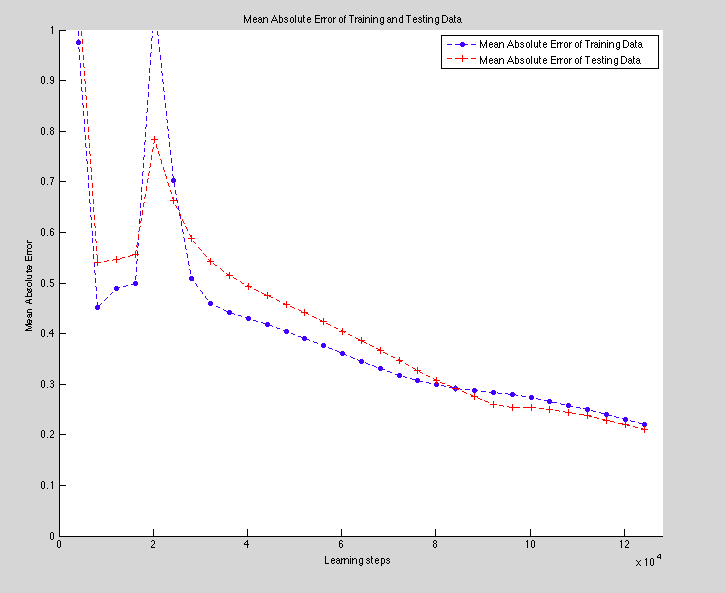
\includegraphics[scale=0.4]{pic1.png}\\
\end{center}
From the plot above, we can see that both for the testing and training errorr, as the simunlation progresses, the errors are decreasing. This is good as it is indicating that both the simulation is learning and that it is not overfitting, a fact that is confirmed in the next plot.\\
\textbf{Final Output}
\begin{center}
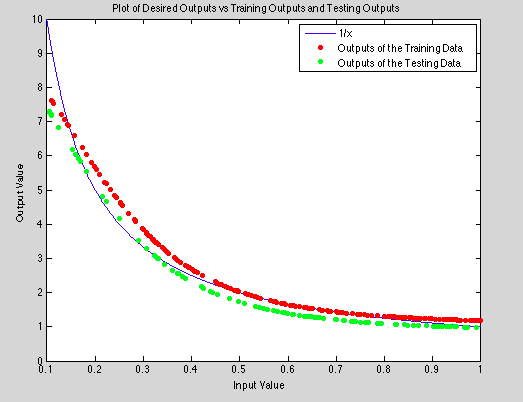
\includegraphics[scale=0.6]{pic2.png}
\end{center}
In this plot we can see that the Neural Network seems to have learned a fair job of learning the 1/x function. A few things to note is that as the input value decreases, the accuracy of the neural network decreases. This is beacuse there is much more variation in the Output Value when the Input Value is small rather than larger making it hard for the NN to learn the correct rules. We also have, as expected, that the Training Data has a lower Average Error 0.1993, than the average error of the Testing Data 0.2545.  And appropriately, the Training Data seems to be better learning 1/x than the Testing Data. But the closeness of the two lines seems to indicate that the NN has not overfitted. 
\newpage
 \section*{HW Part II}
 \subsection*{Problem 3}
 For the simulations following, this will be the base parameters. When one parameter value is going to be changed, it will be assumed that all of the others will be staying constant unless otherwise specified. All simulations were also conducted with the seed value set to a constant to make for easier comparison of parameters.
 \begin{table}[htbp] 
\center
\caption{Parameters of Training BP Network to Fit $f(x) = 1/x$}
  \label{tab:NP}
  %\scalebox{0.9}{ % You can scale the size of the table by changing this number
   \scalebox{1.0}{
   \begin{tabular}{p{4cm} p{.05cm} p{8cm}}
\toprule
  \multicolumn{3}{l}{\bf Network parameters} \\
\bottomrule \noalign{\smallskip}
  Topology & & $(1 + 1_{Bias})$ --- $(10 + 1_{Bias})$ --- $1$ \\
  Transfer function & & Hyperbolic Tangent with slope of 1 \\
\toprule
  \multicolumn{3}{l}{\bf Learning parameters} \\
\bottomrule \noalign{\smallskip}
  Initial weights & & drawn from U[-0.1, 0.1] \\
  Learning rate ($\alpha$) & & 0.01\\
  Momentum & & 0.5\\
  Epoch size ($Epoch$)& &  200 \\
  Stopping criteria & &  error ($Err_{stop}$) $ \le 0.01 $ OR  learn count (t) $ > 600,000 $\\
  Error measure ($Err_{stop}$)& & $\|D^k-y^k\|$ averaged over all training samples\\\toprule
 \multicolumn{3}{l}{\bf Input / output data, representation, scaling} \\
\bottomrule \noalign{\smallskip}
  \# training samples ($N_{tr}$)& & 200 (x values drawn randomly from U[0.1,1])\\
  \# test samples ($N_{tst}$)& & 100 (x values drawn randomly from U[0.1,1])\\
  Scaling of inputs & &  None \\
  Scaling of outputs & &  map [global min, global max] to [-0.75,0.75] \\
%  %\# learn steps performed & & 180,365 (error threshold reached)\\
\toprule
  \multicolumn{3}{l}{\bf Parameters and error measures for performance evaluation} \\
\bottomrule \noalign{\smallskip}
  Error of fit ($Err_{fit}$) & & $\|D^k-y^k\|$ averaged over all testing samples \\
  Final Error of fit for Testing Data && 0.0999\\
  Final Error of fit for Training Data && 0.1210\\
  \# learn steps performed & & 118600 (threshold for $Err_{stop}$ reached)\\
  Monitoring frequency ($m$) & &  200 learning steps\\

 \bottomrule \noalign{\smallskip}
 
  \end{tabular}
   } % end scalebox
\end{table}

\subsection*{Number of PEs}
\begin{center}
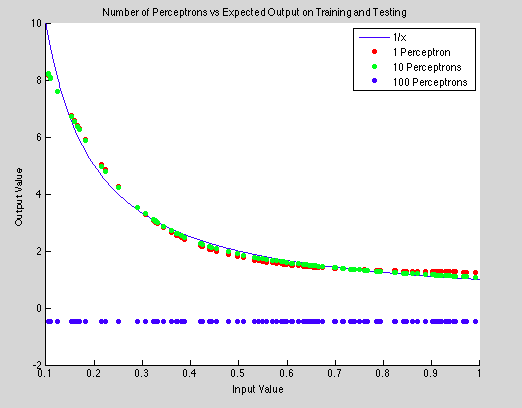
\includegraphics[scale=0.8]{pic3}
\end{center}
In the plots above, the number of perceptrons were varied between 1,10, and 100. It was perhaps unsuprising that when the number of Perceptrons was increased to a large number like 100, the paramters that lead to convergence for 10 would no longer hold because, like Widow's rule of thumb implies, as the number of perceptrons is increased more training data is needed for the network to achieve the same error rate. As for 1 and 10, they both seem to predict similar values, but their differences lies in the speed of convergence.
\begin{center}
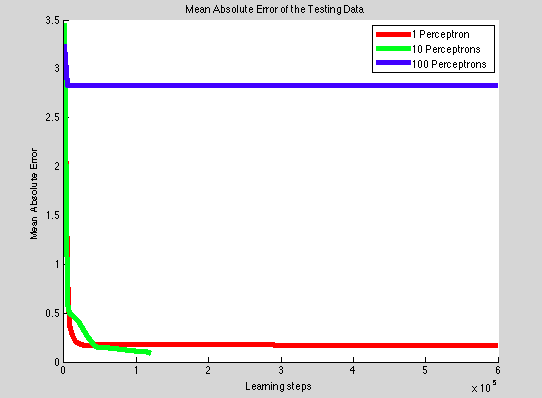
\includegraphics[scale=0.4]{pic4}
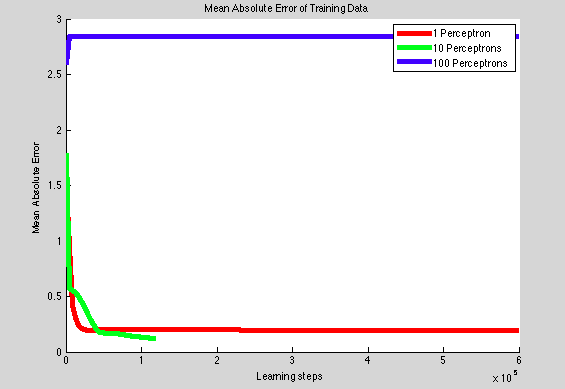
\includegraphics[scale=0.4]{pic4b}
\end{center}
When the number of perceptrons is only one, the NN converges very quickly for both the training and testing data, but due to the limitations of only having one perceptron, it never converges to less than the stopping criteria, 0.01, so it finishes all 600,000 learning steps without getting close to 0.01. Intuitively this makes good sense as it is much quicker to train 1 perceptron than 10. But the paucity makes it hard to learn the data correctly. At 10 perceptrons however, the parameters seem to be just right so that the ANN converges to the correct value. It does this in 118,600 learning steps, a mere 20 percent of the total allotted steps. But at 100, things become even worse. With so many perceptrons, the ANN is having a hard time changing values in a meaningful way. So the Error seems to be stuck at just shy of 3. This seems to indicate that there is a sweet spot for the number of perceptrons inbetween 1 and 1000--A statement that is proved in the next table
\begin{center}
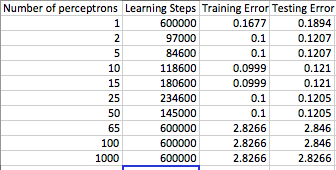
\includegraphics[scale=0.7]{pic5}
\end{center}
As seen in the table, as the number of perceptrons increases, the learning time tends to increase up until a point at which it will no longer converge to the correct value and instaed it will converge to another local minima. The one exception to this is when you have only 1 perceptron in which case, it will not converge, hinting that there are jobs that where only one perceptron will not do. So in general, the number of perceptrons must not be too large or too small. So for our cases, 2 seems to be the best.
\subsection*{Momentum}
 \begin{center}
 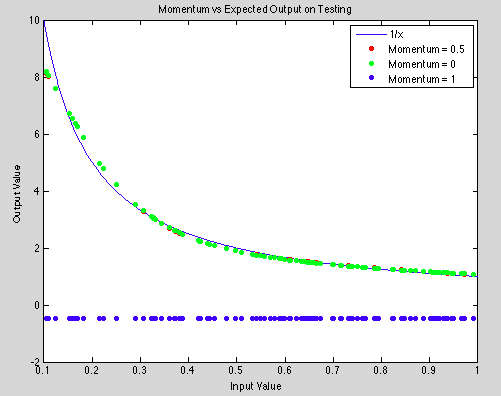
\includegraphics[scale=0.6]{pic6}
 \end{center}
 From this plot, we can see that the momentum term does not seem to have an effect on the convergence if it is inbetween 0.5 and 0. But when momentum is turned to 1, then it seems the NN starts to converge to a different value. Seemingly the same value as when the number of perceptrons was brought to 100.
 
 \begin{center}
 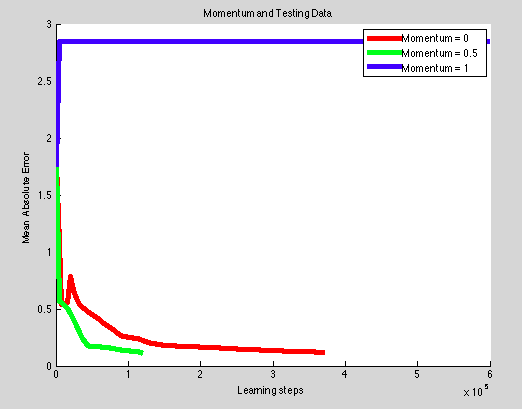
\includegraphics[scale=0.45]{pic7}
 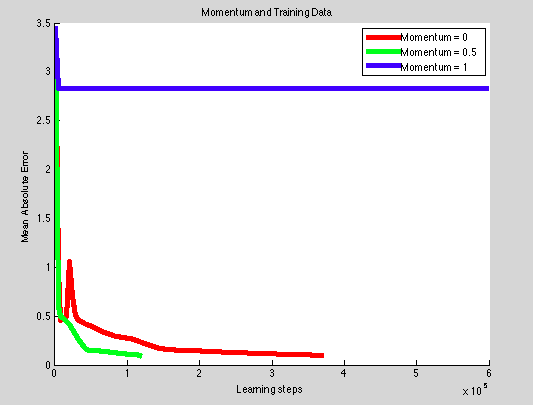
\includegraphics[scale=0.45]{pic7a}
 \end{center}
 Like in Number of Perceptrons, it seems like there is a sweet spot for momentum. When there is no momentum, the operation converges but takes longer than when there is a little bit of momentum. But when there is too much momentum, it seems like the function diverges. This trend is further explored in the table
 \begin{center}
 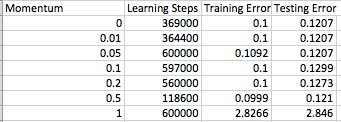
\includegraphics[scale=0.7]{pic8}
 \end{center}
 Interestingly, the relationship here does not seem to be linear like the number of perceptrons. By what seems to be pure coincidence, the originally chosen momentum value of 0.5 seems to be the best as it converges in a fraction of the learning steps that the other ones take. This meas that when it comes to momentum, it seems best to run thourgh arbitrary values until you find a good one.
 \newpage
 \subsection*{Best Results}
 By taking the best parameters from the pervious sections, 0.5 momentum and 2 perceptrons, I was able to create an ANN that was better than any of the previous ones.
 \begin{center}
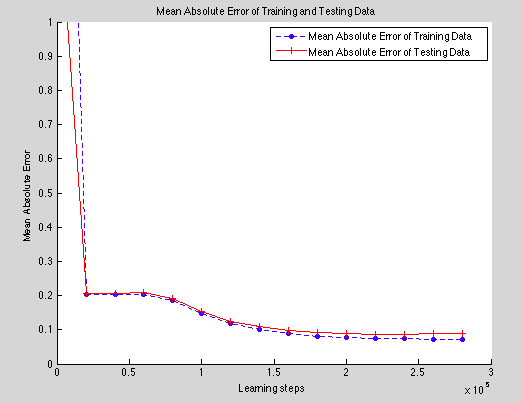
\includegraphics[scale=0.45]{pic11}
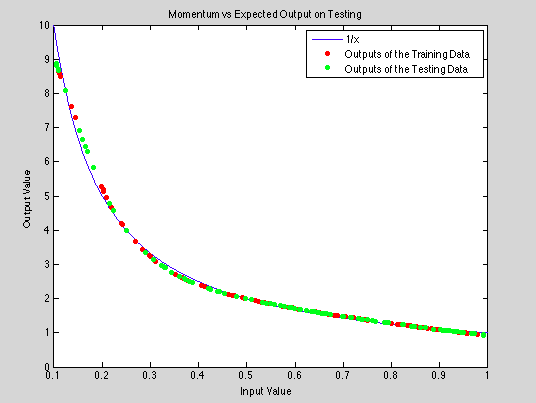
\includegraphics[scale=0.45]{pic12}
 \end{center}
 As we can see on the plot on the left, the outputs of the ANN are nearly identical to the true 1/x function. It seems to overestimate around 0.2 and underestimate around 0.4, but overall, this is by far the best output I have been able to produce. Moreover, from both plots, we can see that the training error and the testing error are nearly identical (difference = 0.0165) meaning that the ANN has not overfitted. Moreover, the table below shows that the ANN managed to learn this is an admittedly large number of learning steps, but was able to obtain an average error of 0.0729 to 0.0894. Meaning that the ANN would output a quess that is on average not more than 0.08 from the true value--overally a pretty accurate algorithmn. \\
\begin{center}
 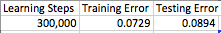
\includegraphics[scale=1]{pic13}
\end{center}
  
 \subsection*{Problem 4}
 \begin{table}[htbp] 
\center
\caption{Parameters of Training BP Network to Fit Iris Data Set}
  \label{tab:NP}
  %\scalebox{0.9}{ % You can scale the size of the table by changing this number
   \scalebox{1.0}{
   \begin{tabular}{p{4cm} p{.05cm} p{8cm}}
\toprule
  \multicolumn{3}{l}{\bf Network parameters} \\
\bottomrule \noalign{\smallskip}
  Topology & & $(1 + 1_{Bias})$ --- $(10 + 1_{Bias})$ --- $1$ \\
  Transfer function & & Hyperbolic Tangent with slope of 1 \\
\toprule
  \multicolumn{3}{l}{\bf Learning parameters} \\
\bottomrule \noalign{\smallskip}
  Initial weights & & drawn from U[-0.1, 0.1] \\
  Learning rate ($\alpha$) & & 0.02\\
  Momentum & & 0.5\\
  Epoch size ($Epoch$)& &  200 \\
  Stopping criteria & &  error ($Err_{stop }$) $ \le 0.04 $ OR  learn count (t) $ > 225,000$\\
  Error measure ($Err_{stop}$)& & $ Acc_X = \frac{\# correct\enspace hits}{|X|}\enspace \%$ See formula (2) below \\\toprule
 \multicolumn{3}{l}{\bf Input / output data, representation, scaling} \\
\bottomrule \noalign{\smallskip}
  \# training samples ($N_{tr}$)& & 75 \\
  \# test samples ($N_{tst}$)& & 75 \\
  Scaling of inputs & &  None \\
  Scaling of outputs & &  None \\
%  %\# learn steps performed & & 180,365 (error threshold reached)\\
\toprule
  \multicolumn{3}{l}{\bf Parameters and error measures for performance evaluation} \\
\bottomrule \noalign{\smallskip}
  Error of fit ($Err_{fit}$) & & $ Acc_X = \frac{\# correct\enspace hits}{|X|}\enspace \%$\\
  Final Error of fit for Testing Data &&  0.0267\\
  Final Error of fit for Training Data && 0.0400\\
  \# learn steps performed & & 1,725 (threshold for $Err_{stop}$ reached)\\
  Monitoring frequency ($m$) & &  150 learning steps\\
 \bottomrule \noalign{\smallskip}
   \end{tabular}
   } 
\end{table}
 To transition to the Iris dataset, a few modifications were necessary. First was a change in Error measure from mean absolute error to classification accuracy. Specifically, the concept of a correct hit had to be established. Designating an output $y^k$ to be giving the correct response only when $y^k = D^k$ did not lead to any form of convergence. Hence, the following function was applied to the outputs. \\
 \newline
 Let $D_y^k = \min (d_1^k, d_2^k, d_3^k)$. Where $d_1^k$ is the distance from $y^k$ to [1,0,0], $d_2^k$ is from $y^k$ to $[0,1,0]$, and $d_3 ^ k$ is the euclidean distance to $[0,0,1]$, the thresholded output, $\hat{y^k}$ is equal to $[1,0,0]$ if $D_y^k = d_1 ^k$, $[0,1,0]$ if $D_y^k = d_2 ^k$, and $[0,0,1]$ if $D_y^k = d_3 ^k$. Ie it maps every output to the closest possible output. Then when, $\hat{y^k} = D^k$, we would designate this as a correct hit.\\
 \newline
 So in summary, an output is a correct hit if the point that is closest to the output is the desired output. When another possible point is closer, it is an incorrect hit.\\
 \newline
 \textbf{Route to the Final Parameters}\\
 At first, the simulation was run with parameter values that were identical to those in the previous question. However, after remembering that the slides shown in class about Widow's rule and the VC indicated that 75 datapoints is too few even for 2 perceptrons, the number of perceptrons was decreased from 10 to 2. Then after a bit of trial and error with random learning rates, the following results were produced.\\
 \textbf{Learning History}\\
\begin{center}
 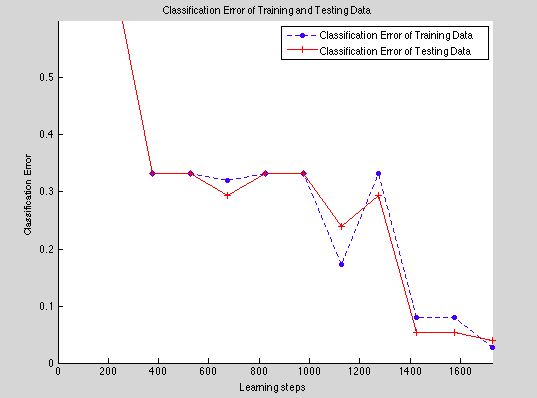
\includegraphics[scale=0.7]{pic9.png}
\end{center}
From the plot above, we can see that the ANN is indeed learning the Iris Data--both the training and testing error are decreasing. And it seems to have a converged to a very low error of 0.03
\begin{center}
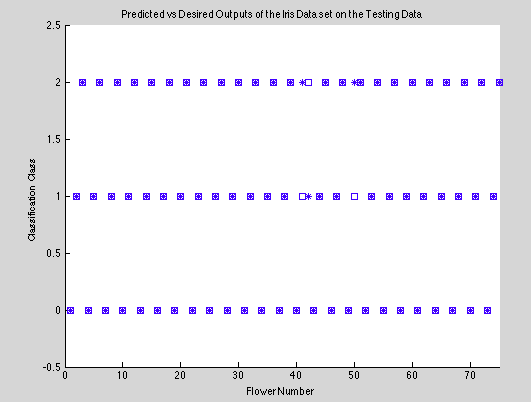
\includegraphics[scale=0.7]{pic10.png}
\end{center}
This plot above shows which category each flower was in vs what the ANN thought it should have been in. Every box represents the category that the flower was in with height = 0 being Setosa, height = 1 being Versacolor and  height = 3 being Virginica.  Each asterisk represents which category the ANN thought the flower should be in. As we can see the ANN was perfect with heigh =0, the Setosa, but it had issues with the Versacolor and especially the Virgincia. So with only 3 miscategorizations out of 75, or an error of 4 percent, the ANN seems to be a good tool for categorizing the iris dataset.

\end{document}